\documentclass[letterpaper,10pt,onecolumn]{article}
\usepackage[spanish]{babel}
\usepackage[utf8x]{inputenc}
\usepackage{amsfonts}
\usepackage{amsthm}
\usepackage{amsmath}
\usepackage{mathrsfs}
\usepackage{empheq}
\usepackage{enumitem}
\usepackage[pdftex]{color,graphicx}
\usepackage{hyperref}
\usepackage{listings}
\usepackage{calligra}
\usepackage{algpseudocode} 
\DeclareMathAlphabet{\mathcalligra}{T1}{calligra}{m}{n}
\DeclareFontShape{T1}{calligra}{m}{n}{<->s*[2.2]callig15}{}
\newcommand{\scripty}[1]{\ensuremath{\mathcalligra{#1}}}
\lstloadlanguages{[5.2]Mathematica}
\setlength{\oddsidemargin}{0cm}
\setlength{\textwidth}{490pt}
\setlength{\topmargin}{-40pt}
\addtolength{\hoffset}{-0.3cm}
\addtolength{\textheight}{4cm}

\begin{document}
\begin{center}



\includegraphics[width=490pt]{header.png}\\[0.5cm]

\textsc{\LARGE Taller 3 - F\'isica I (FISI-1018) - 2016-10}\\[0.5cm]

\textsc{\Large{Profesor: Jaime Forero}} \\[0.5cm]

\noindent\textsc{Ejercicios correspondiente a la clase complementaria de la semana del 8 de Febrero del 2016.}\\[0.5cm]
\end{center}

\noindent\textsc{Nota:} 
Los primeros tres ejercicios deben ser
entregados {\bf al comienzo} de la clase complementaria. Los \'ultimos
cuatro deben ser trabajados {\bf durante} la complementaria. 

La numeraci\'on
hace referencia al texto gu\'ia: \textit{F\'isica Universitaria Volumen
  1 (Sears-Semansky)}, decimotercera edici\'on, Pearson.

\begin{enumerate}
% aqui vienen los tres ejercicios "faciles"
\item Ejercicio 3.10 Intr\'epida nadadora.
\item Ejercicio 3.25 Rotaci\'on de la Tierra.
\item Problema 3.49 Cuadrilla de demolici\'on.

% aqui vienen los cuatro ejercicios "dificiles"
\item Ejercicio 3.71 Roca lanzada sobre una represa. %propuesto por Juan Carlos

\item Una centrifugadora de la NASA en el {\it Ames Research
Center} en Mountain View, California, esta formada por un cilindro de 20 metros de longitud disopuesto de forma horizontal, como se muestra en la figura. Asumiendo que un astronauta está sentado en la silla de uno de los extremos, determine la tasa de rotación, en revoluciones por segundo, que se requiere para que la aceleración centrípeta sobre el astronauta sea de 20 veces $g$.

\begin{figure}[h]
\centering
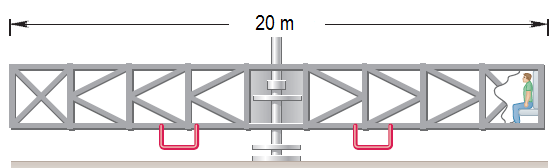
\includegraphics[width=0.8\textwidth]{astronauta.PNG}
\caption{Centrifugadora en el {\it Ames Research Center}}
\end{figure}


\item
Un cañon, situado a $60m$ del borde de un risco vertical de $25m$ de altura, dispara un proyectil de 15kg con un angulo de $45^{\circ}$ sobre la horizontal, hacia el risco.
\begin{enumerate}
\item Realice una gráfica del problema, indicando como se mueve el proyectil.
\item ¿Qué velocidad inicial debe tener el proyectil para pasar el borde del risco?
\item ¿Qué distancia recorre el proyectil?. ¿A que distancia del borde del risco cae el proyectil?
\end{enumerate} 

 %propuesto por Miguel


\item
Un modelo de rotor de helicóptero tiene cuatro aspas, cada una de $3.4m$ de longitud desde el eje central hasta la punta. El modelo gira en un túnel de viento a $550rpm$
\begin{enumerate}
\item 
¿Qué rapidez lineal tiene la punta del aspa en $m/s$?
\item
¿Qué aceleración radial tiene la punta del aspa, expresada como múltiplo de la aceleración debida a la gravedad $g$?
\end{enumerate}
\end{enumerate}

\newpage

{\bf Ejercicios recomendados como preparaci\'on para el parcial}\\

\begin{enumerate}
\item Una part\'icula se mueve en un plano de tal manera que su
  posici\'on en funci\'on del tiempo es $\vec{r}(t)= 5t\hat{i} +
  5t(1-2t)\hat{j}$ donde las distancias est\'an medidas en metros y
  los tiempos en segundos. 

\begin{itemize}
\item Encuentre la velocidad de la part\'icula en funci\'on
  del tiempo. 
\item  Encuentre la aceleraci\'on en funci\'on del tiempo. 
\item Encuentre la rapidez m\'inima que alcanza la
  part\'icula.   
\end{itemize}

\item Una bola de lana parte del reposo en ca\'ida libre
  desde una altura de $10$ metros. Al mismo tiempo que la bola empieza a caer un gato que est\'a ubicado justo por debajo salta hacia arriba para atraparla. El gato tiene una
  velocidad inicial de $10$ metros por segundo. ¿A qu\'e altura, medida desde el suelo, va a atrapar el gato a la bola de lana?

\item Una manera de medir la acelaraci\'on de la gravedad es lanzar
  alg\'un objeto hacia arriba y medir el tiempo que pasa en cruzar dos
  puntos diferentes en las dos direcciones. Muestre que si 
  $T_A$ es el tiempo que le toma al objeto pasar una l\'inea horizonal
  $A$ en ambas direcciones, y $T_B$ es el tiempo que le toma para pasar en dos
  direcciones por   otra l\'inea $B$, entonces la aceleraci\'on de la
  gravedad est\'a dada por:
  \begin{displaymath}
    g = \frac{8h}{T_A^2 -T_B^2}.
  \end{displaymath}
  Nota: ver la Figura \ref{fig:tiro}. 

\item El Hyperloop es el nombre de un proyecto de un tren de alta velocidad que va a conectar las ciudades de Los \'Angeles y San Francisco en California. En la Figura \ref{fig:tiro} vemos lo que se planea tener para la velocidad (en millas por hora) como funci\'on del tiempo (en segundos) medido deesde el comienzo del viaje en Los \'Angeles hasta su destino. 
\begin{itemize}
\item Seg\'un la gr\'afica ¿Cu\'antos minutos durar\'a un
  viaje en el Hyperloop? 
\item Estime a partir de la gr\'afica la distancia (expresada en kil\'ometros) recorrida por el Hyperloop entre Los \'Angeles y San Francisco.  1 milla equivale a 1.60 kil\'ometros. 
\end{itemize}

\end{enumerate}

\begin{figure}[!h]
\begin{center}
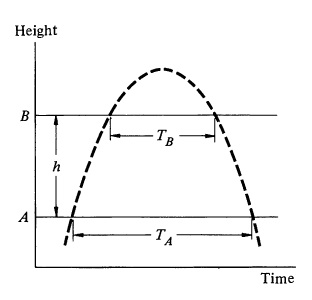
\includegraphics[scale=0.6]{altura.jpg} 
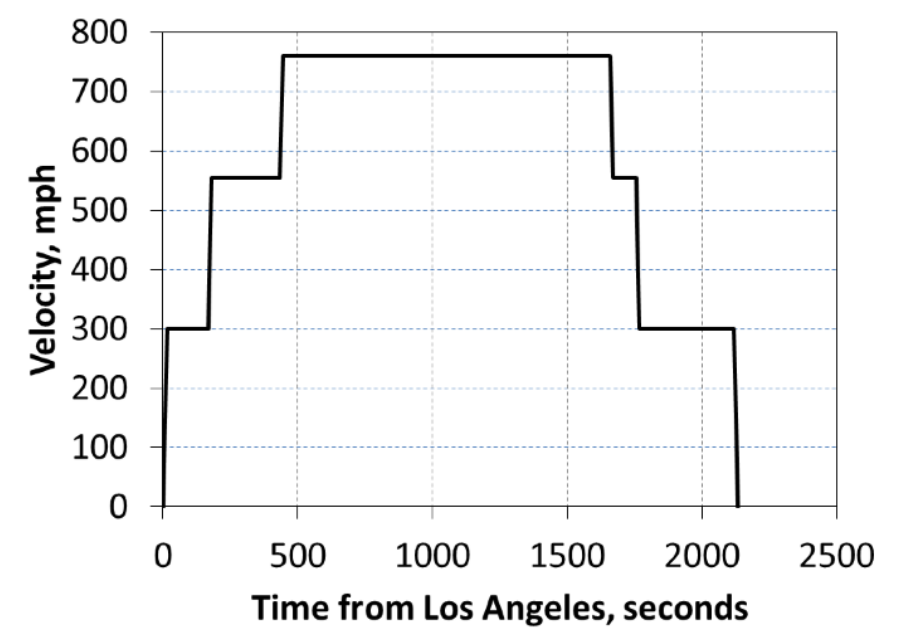
\includegraphics[scale=0.3]{hyperloop.png} 
\end{center}
\caption{Izquierda: diagrama para el ejercicio recomendado 3. Derecha: diagrama para el ejercicio recomendado 4.} 
\label{fig:tiro}
\end{figure}






\end{document}
